\documentclass[border=4pt,12pt]{standalone}
% House style for redrawn exam diagrams (diagram-v4: 0.4pt lines, filled -latex arrows, fine dashes; stipple and hatching drawn as real dots/lines (no PDF/SVG patterns, so they render in every browser and at any scale); transparent background). Every figure \input's this.
\usepackage{amsmath,amssymb}
\usepackage{txfonts}
\usepackage{pdfrender,xcolor}
% \halo{text}: label on shading. The shading stops just around each letter's outline (a thin knock-out that follows the
% glyphs, like the papers' typesetting), never a box. Owner: "I don't want a box around the text".
\newcommand{\halo}[1]{\leavevmode\rlap{\pdfrender{TextRenderingMode=2,LineWidth=2.2pt,LineJoinStyle=1,StrokeColor=white,FillColor=white}#1}#1}
\usepackage{tikz,pgfplots}
\pgfplotsset{compat=1.18}
\usetikzlibrary{arrows.meta,calc,angles,quotes,patterns,patterns.meta,intersections,positioning,decorations.markings,shapes.geometric}
% Stipple and hatching are drawn as actual dots / lines clipped to the region (path picture), NOT as pattern fills:
% SVG <pattern> fills vanish or blur when browsers scale the image, so the owner could not see the shading.
% Each dot is a 0.72pt square (keeps SVGs small; reads as a dot at print size). Dots sit on one global staggered grid, so neighbouring regions line up.
\makeatletter
\newdimen\ex@x \newdimen\ex@y \newdimen\ex@xa \newdimen\ex@ya \newdimen\ex@xb \newdimen\ex@yb \newcount\ex@row
\def\exam@stipplecolor{black!75}\def\exam@dotr{0.42pt}\def\exam@dotgap{2.5}
\def\ex@rowdots{\ifdim\ex@x<\ex@xb \pgfpathrectangle{\pgfqpoint{\dimexpr\ex@x-0.36pt\relax}{\dimexpr\ex@y-0.36pt\relax}}{\pgfqpoint{0.72pt}{0.72pt}}\advance\ex@x by \exam@dotgap pt\relax\expandafter\ex@rowdots\fi}
\def\exam@stipple{%
  \pgftransformreset% dots are sized in real points even inside scaled pictures
  \pgfpointanchor{path picture bounding box}{south west}\ex@xa=\pgf@x \ex@ya=\pgf@y
  \pgfpointanchor{path picture bounding box}{north east}\ex@xb=\pgf@x \ex@yb=\pgf@y
  \pgfsetfillcolor{\exam@stipplecolor}\pgfmathsetmacro\ex@h{\exam@dotgap/2}%
  \pgfmathtruncatemacro\ex@r{floor(\ex@ya/\ex@h)-1}\ex@row=\ex@r\relax
  \ex@y=\ex@r\dimexpr\ex@h pt\relax
  \loop\ifdim\ex@y<\ex@yb
    \pgfmathtruncatemacro\ex@c{floor(\ex@xa/\exam@dotgap)-1}\ex@x=\ex@c\dimexpr\exam@dotgap pt\relax
    \ifodd\ex@row \advance\ex@x by \ex@h pt\fi
    \ex@rowdots
    \advance\ex@y by \ex@h pt \advance\ex@row by 1
    \ifnum\numexpr\ex@row-(\ex@row/4)*4\relax=0 \pgfusepath{fill}\fi% flush every 4 rows: bounded TeX memory, few clip copies in the SVG
  \repeat\pgfusepath{fill}}
\newdimen\ex@d
\def\exam@hatch#1{% #1 = 1 for /, -1 for \ ; lines 45 degrees, 3pt apart
  \pgftransformreset
  \pgfpointanchor{path picture bounding box}{south west}\ex@xa=\pgf@x \ex@ya=\pgf@y
  \pgfpointanchor{path picture bounding box}{north east}\ex@xb=\pgf@x \ex@yb=\pgf@y
  \ex@d=\dimexpr\ex@yb-\ex@ya\relax \ex@x=\dimexpr\ex@xa-\ex@d\relax
  \loop\ifdim\ex@x<\ex@xb
    \ifnum#1>0 \pgfpathmoveto{\pgfqpoint{\ex@x}{\ex@ya}}\pgfpathlineto{\pgfqpoint{\dimexpr\ex@x+\ex@d\relax}{\ex@yb}}%
    \else \pgfpathmoveto{\pgfqpoint{\ex@x}{\ex@yb}}\pgfpathlineto{\pgfqpoint{\dimexpr\ex@x+\ex@d\relax}{\ex@ya}}\fi
    \advance\ex@x by 4.24pt
  \repeat
  \pgfsetlinewidth{0.4pt}\pgfsetstrokecolor{black}\pgfusepath{stroke}}
\def\examstipple{\exam@stipple}\def\examhatch{\exam@hatch}\def\examsetstipplecolor#1{\def\exam@stipplecolor{#1}}\def\examsetdotgap#1{\def\exam@dotgap{#1}}
\makeatother
% (legacy pattern kept for old files)
% staggered stipple like the NESA papers' dotted shading
\pgfdeclarepatternformonly{exam stipple}{\pgfpointorigin}{\pgfqpoint{2.2pt}{2.2pt}}{\pgfqpoint{2.2pt}{2.2pt}}{%
  \pgfpathcircle{\pgfqpoint{0.55pt}{0.55pt}}{0.42pt}\pgfpathcircle{\pgfqpoint{1.65pt}{1.65pt}}{0.42pt}\pgfusepath{fill}}
\tikzset{
  every picture/.style={line width=0.6pt, >={Latex[length=2mm,width=1.3mm]}},
  curve/.style={line width=0.6pt},
  open arrow/.style={-{Latex[length=2mm,width=1.3mm]}},  % owner: filled -latex heads everywhere, no open chevrons
  aux/.style={dash pattern=on 2pt off 1.5pt, line width=0.6pt},
  shade/.code={\def\exA{#1}\def\exB{none}\ifx\exA\exB\else\pgfkeysalso{fill=black!18}\fi},
  shade/.default=on,
  shade dots/.style={fill=none, path picture={\examstipple}},
  stipple color/.code={\examsetstipplecolor{#1}},
  stipple gap/.code={\examsetdotgap{#1}},
  shade dense dots/.style={fill=none, stipple gap=1.6, path picture={\examstipple}},
  shade hatch/.style={fill=none, path picture={\examhatch{1}}},
  shade hatch reverse/.style={fill=none, path picture={\examhatch{-1}}},
  shade solid/.style={fill=black},
  pt/.style={circle, fill, inner sep=1.1pt},
  open pt/.style={circle, draw, fill=white, inner sep=1.1pt},
}
\pgfplotsset{
  exam axes/.style={axis lines=middle, axis line style={->}, xlabel={$x$}, ylabel={$y$},
    xlabel style={anchor=west}, ylabel style={anchor=south}, tick label style={font=\small},
    every axis plot/.append style={line width=0.6pt, black}, samples=200, clip=false,
    enlargelimits=false, axis on top},
}

\begin{document}
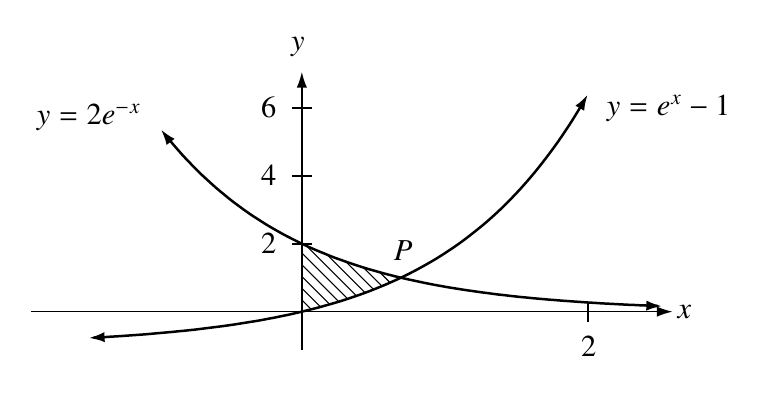
\begin{tikzpicture}[x=0.0127cm,y=-0.0127cm, every node/.style={font=\fontsize{11}{13}\selectfont}]
\fill[shade hatch reverse] plot[smooth] coordinates {(301.0,217.0) (306.2,219.4) (311.4,221.8) (316.7,224.0) (321.9,226.2) (327.1,228.3) (332.3,230.4) (337.5,232.3) (342.7,234.2) (348.0,236.0) (353.2,237.8) (358.4,239.5) (363.6,241.1) (368.8,242.7) (374.0,244.2) (379.3,245.7) (384.5,247.1) (389.7,248.4) (394.9,249.7) (400.1,251.0)} -- plot[smooth] coordinates {(400.1,251.0) (394.9,253.4) (389.7,255.8) (384.5,258.0) (379.3,260.2) (374.0,262.3) (368.8,264.4) (363.6,266.3) (358.4,268.2) (353.2,270.0) (348.0,271.8) (342.7,273.5) (337.5,275.1) (332.3,276.7) (327.1,278.2) (321.9,279.7) (316.7,281.1) (311.4,282.4) (306.2,283.7) (301.0,285.0)} -- cycle;
\draw[->] (30,285) -- (672,285);
\draw[->] (301,323) -- (301,45);
\draw (291,217.0) -- (311,217.0);
\draw (291,149.0) -- (311,149.0);
\draw (291,81.0) -- (311,81.0);
\draw (587.0,275) -- (587.0,295);
\draw[<->,line width=0.9pt] plot[smooth] coordinates {(160.0,102.7) (165.6,109.8) (171.3,116.5) (176.9,123.0) (182.5,129.3) (188.2,135.3) (193.8,141.1) (199.4,146.7) (205.1,152.0) (210.7,157.1) (216.3,162.1) (222.0,166.8) (227.6,171.4) (233.2,175.8) (238.9,180.0) (244.5,184.1) (250.1,188.0) (255.8,191.7) (261.4,195.3) (267.0,198.8) (272.7,202.1) (278.3,205.3) (283.9,208.4) (289.6,211.3) (295.2,214.2) (300.8,216.9) (306.5,219.6) (312.1,222.1) (317.7,224.5) (323.4,226.8) (329.0,229.1) (334.6,231.3) (340.3,233.3) (345.9,235.3) (351.5,237.2) (357.2,239.1) (362.8,240.9) (368.4,242.6) (374.1,244.2) (379.7,245.8) (385.3,247.3) (391.0,248.8) (396.6,250.2) (402.2,251.5) (407.9,252.8) (413.5,254.0) (419.1,255.2) (424.8,256.4) (430.4,257.5) (436.0,258.6) (441.7,259.6) (447.3,260.6) (452.9,261.5) (458.6,262.4) (464.2,263.3) (469.8,264.1) (475.5,264.9) (481.1,265.7) (486.7,266.4) (492.4,267.2) (498.0,267.9) (503.6,268.5) (509.3,269.2) (514.9,269.8) (520.5,270.4) (526.2,270.9) (531.8,271.5) (537.4,272.0) (543.1,272.5) (548.7,273.0) (554.3,273.4) (560.0,273.9) (565.6,274.3) (571.2,274.7) (576.9,275.1) (582.5,275.5) (588.1,275.9) (593.8,276.2) (599.4,276.6) (605.0,276.9) (610.7,277.2) (616.3,277.5) (621.9,277.8) (627.6,278.1) (633.2,278.3) (638.8,278.6) (644.5,278.8) (650.1,279.1) (655.7,279.3) (661.4,279.5)};
\draw[<->,line width=0.9pt] plot[smooth] coordinates {(87.9,311.3) (93.5,311.0) (99.1,310.7) (104.8,310.4) (110.4,310.0) (116.0,309.7) (121.6,309.3) (127.2,308.9) (132.8,308.5) (138.4,308.1) (144.0,307.7) (149.6,307.2) (155.2,306.7) (160.8,306.2) (166.4,305.7) (172.0,305.2) (177.7,304.6) (183.3,304.1) (188.9,303.5) (194.5,302.9) (200.1,302.2) (205.7,301.5) (211.3,300.8) (216.9,300.1) (222.5,299.4) (228.1,298.6) (233.7,297.8) (239.3,296.9) (244.9,296.0) (250.5,295.1) (256.2,294.2) (261.8,293.2) (267.4,292.1) (273.0,291.1) (278.6,289.9) (284.2,288.8) (289.8,287.6) (295.4,286.3) (301.0,285.0) (306.6,283.6) (312.2,282.2) (317.8,280.8) (323.4,279.2) (329.1,277.6) (334.7,276.0) (340.3,274.3) (345.9,272.5) (351.5,270.6) (357.1,268.7) (362.7,266.7) (368.3,264.6) (373.9,262.4) (379.5,260.1) (385.1,257.8) (390.7,255.3) (396.3,252.8) (402.0,250.1) (407.6,247.4) (413.2,244.5) (418.8,241.5) (424.4,238.4) (430.0,235.2) (435.6,231.9) (441.2,228.4) (446.8,224.7) (452.4,221.0) (458.0,217.1) (463.6,213.0) (469.2,208.7) (474.8,204.3) (480.5,199.7) (486.1,195.0) (491.7,190.0) (497.3,184.9) (502.9,179.5) (508.5,173.9) (514.1,168.1) (519.7,162.1) (525.3,155.8) (530.9,149.3) (536.5,142.5) (542.1,135.4) (547.7,128.1) (553.4,120.4) (559.0,112.5) (564.6,104.2) (570.2,95.7) (575.8,86.7) (581.4,77.4) (587.0,67.8)};
\node at (297,20) {$y$};
\node at (683,285) {$x$};
\node at (588,320) {$2$};
\node at (402,224) {$P$};
\node at (88,90) {$y=2e^{-x}$};
\node at (668,82) {$y=e^x-1$};
\node at (268,217.0) {$2$};
\node at (268,149.0) {$4$};
\node at (268,81.0) {$6$};
\end{tikzpicture}
\end{document}